\chapter{Quantised vortices in droplets}\label{sec:quant-vort}
	\lettrine[lines=4]{\color{activeColor}O}{ne} of the most unambiguous signatures of the quantum mechanical nature of a substance---and indeed superfluidity---is the appearance of quantised vortices. In contrast to a normal fluid, which will rotate as a solid body when its container moves at low angular velocity, a superfluid will remain at rest. However, above a certain critical angular velocity the thermodynamically stable state of a superfluid includes one or more quantum vortices. Such a vortex can be characterised by a macroscopic wave function and quantised velocity circulation in units of $\kappa=\frac{h}{m}$, where $h$ is Planck’s constant and $m$ is the mass of the $^4$He atom\citep{Don91,Pit03}. Recently, the study of vorticity was extended to finite systems such as BECs confined to traps\citep{Pit03,Fetter2009}. The transfer of energy and angular momentum in finite systems between quantised vortices and surface excitations is of particular interest, as it defines the nucleation dynamics, shape, and stability of the involved vortices\citep{Pit03,Fetter2009}. In comparison to confined BECs, $^4$He droplets are self-contained and present a case for the strongly interacting superfluid. Moreover, the diameter of a vortex core which is approximately 0.2 nm in superfluid $^4$He\citep{Don91} is small relative to the droplet size, suggesting a three-dimensionality of the vortices in droplets. Vorticity in $^4$He droplets has therefore attracted considerable interest\citep{Clo98,Lehmann2003,Bar06,Sti06}.
	
	Recently, Gomez \emph{et al}. performed experiments\citep{Gom12} where vortices inside superfluid $^4$He droplets, produced by the expansion of liquid helium, were traced by introducing Ag atoms which clustered along the vortex lines, into the droplets. The helium droplets needed by these kind of experiments need to be larger than used before for single atom spectroscopy and dynamics studies because they need to be be big enough to be able to host an array of vortices, doped with many Ag clusters. A schematic of the experimental principle is shown in \fig{fig:vortex-machine}. Helium droplets are produced by expansion of He, at 20 bar and a temperature $T_0$=5.4--7 K, into vacuum through a nozzle. The droplets cool rapidly via evaporation and reach a temperature of 0.37 K\citep{Hartmann1995}, which is well below the superfluid transition temperature $T_\lambda=2.17\unit{K}$\citep{Don91,Pit03}. Further downstream, the droplets capture 10$^3$–10$^6$ Ag atoms in an oven\citep{Log11d}. The droplets are then collided against a thin carbon film substrate at room temperature\citep{Log11d}. Upon impact, the droplets evaporate, leaving on the surface the Ag traces, which are subsequently imaged via a transmission electron microscope (TEM). The prevalence of elongated track-shaped deposits (see \fig{fig:silver-filament}) shows that vortices are present in droplets larger than about $300\unit{nm}$ and that their lifetime exceeds a few milliseconds.
	
	\begin{figure}[t]
		\begin{center}
			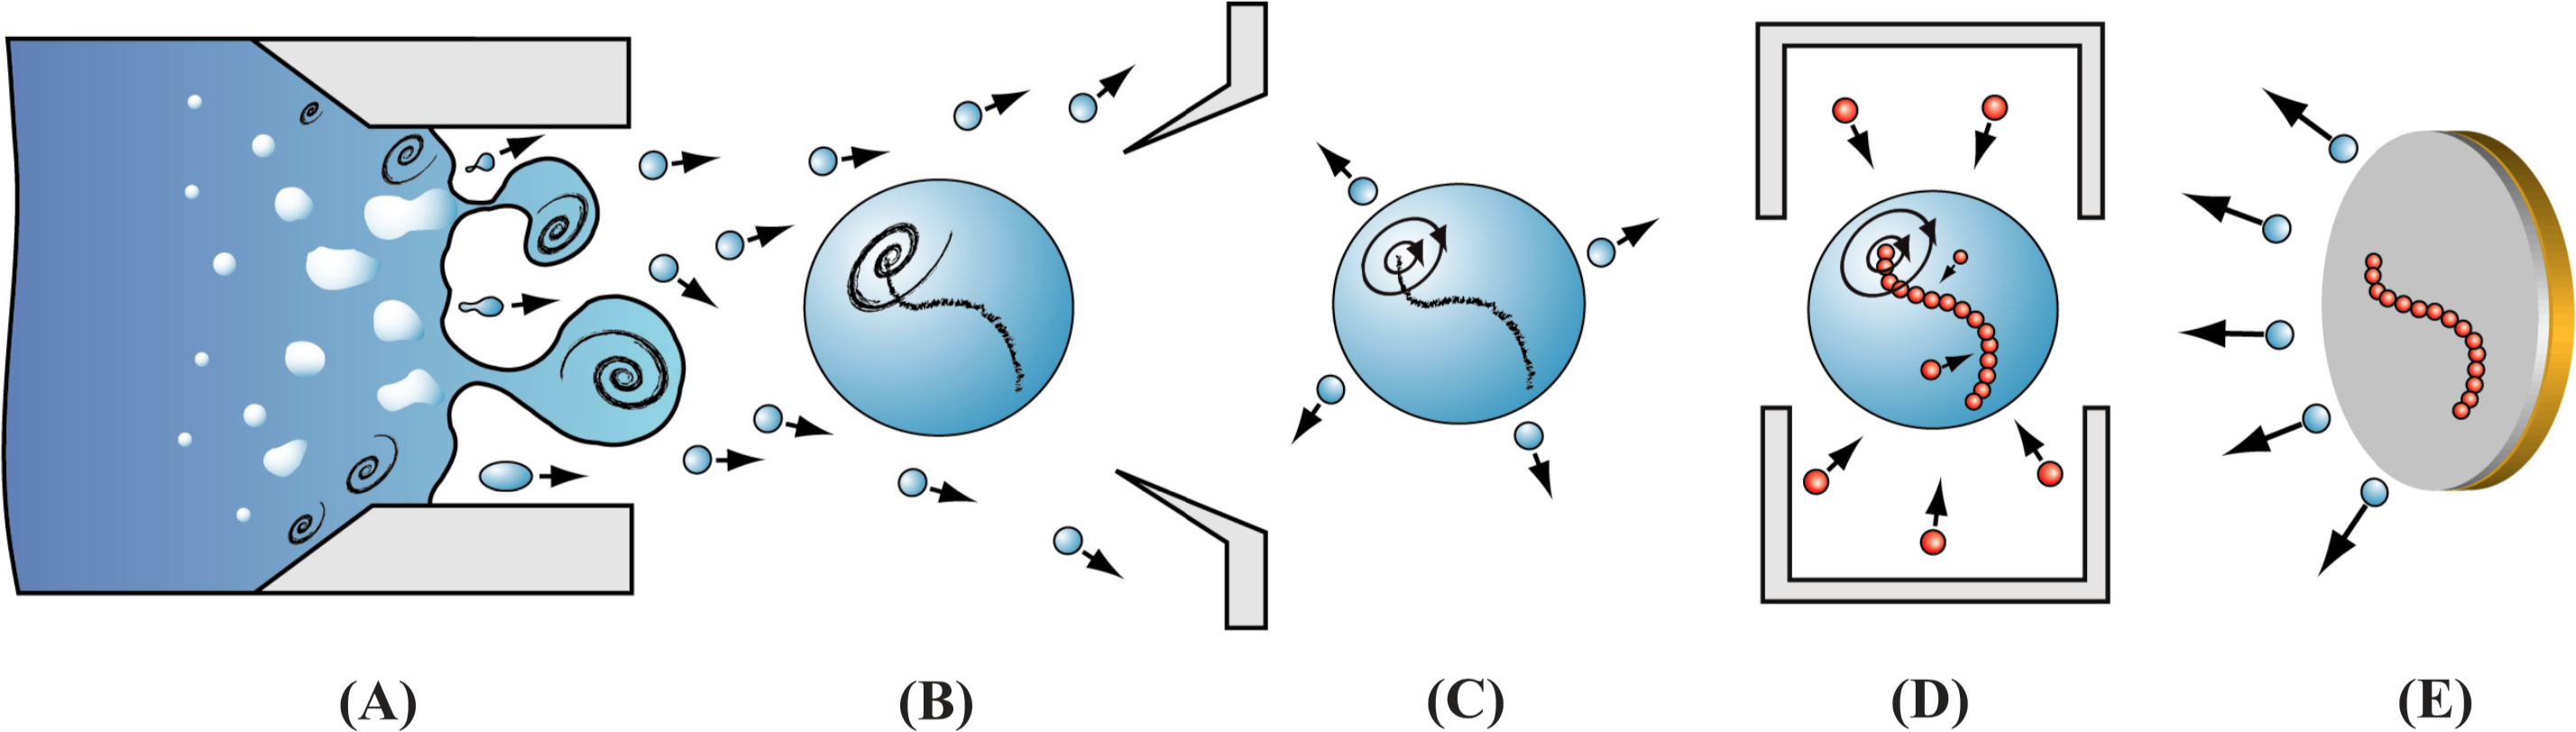
\includegraphics[width=\textwidth]{vortex-machine}
			\caption{Schematic of the experiment. (a) He fluid expands in vacuum and (b) breaks up into rotating droplets. (c) A quantum vortex is formed as a consequence of fast evaporative cooling of the droplet to below $T_\lambda$. (d) The droplet is doped with Ag atoms, which are attracted to the vortex core. (e) The droplet then collides with the carbon surface leaving behind the Ag trace, whereas the He evaporates.}
			\label{fig:vortex-machine}
		\end{center}
	\end{figure}	
	
	Two years later Gomez \emph{et al}. reported\citep{Gom14} on the formation of quantum vortex lattices inside droplets. They used single-shot femtosecond X-ray coherent diffractive imaging to investigate the rotation of single, isolated superfluid helium-4 droplets containing about $10^8$--$10^{11}$ atoms. The formation of quantum vortex lattices inside the droplets was confirmed by observing the characteristic Bragg patterns from xenon clusters trapped in the vortex cores (see \fig{fig:vortex-array}).

	\begin{figure}[t]
		\begin{center}
			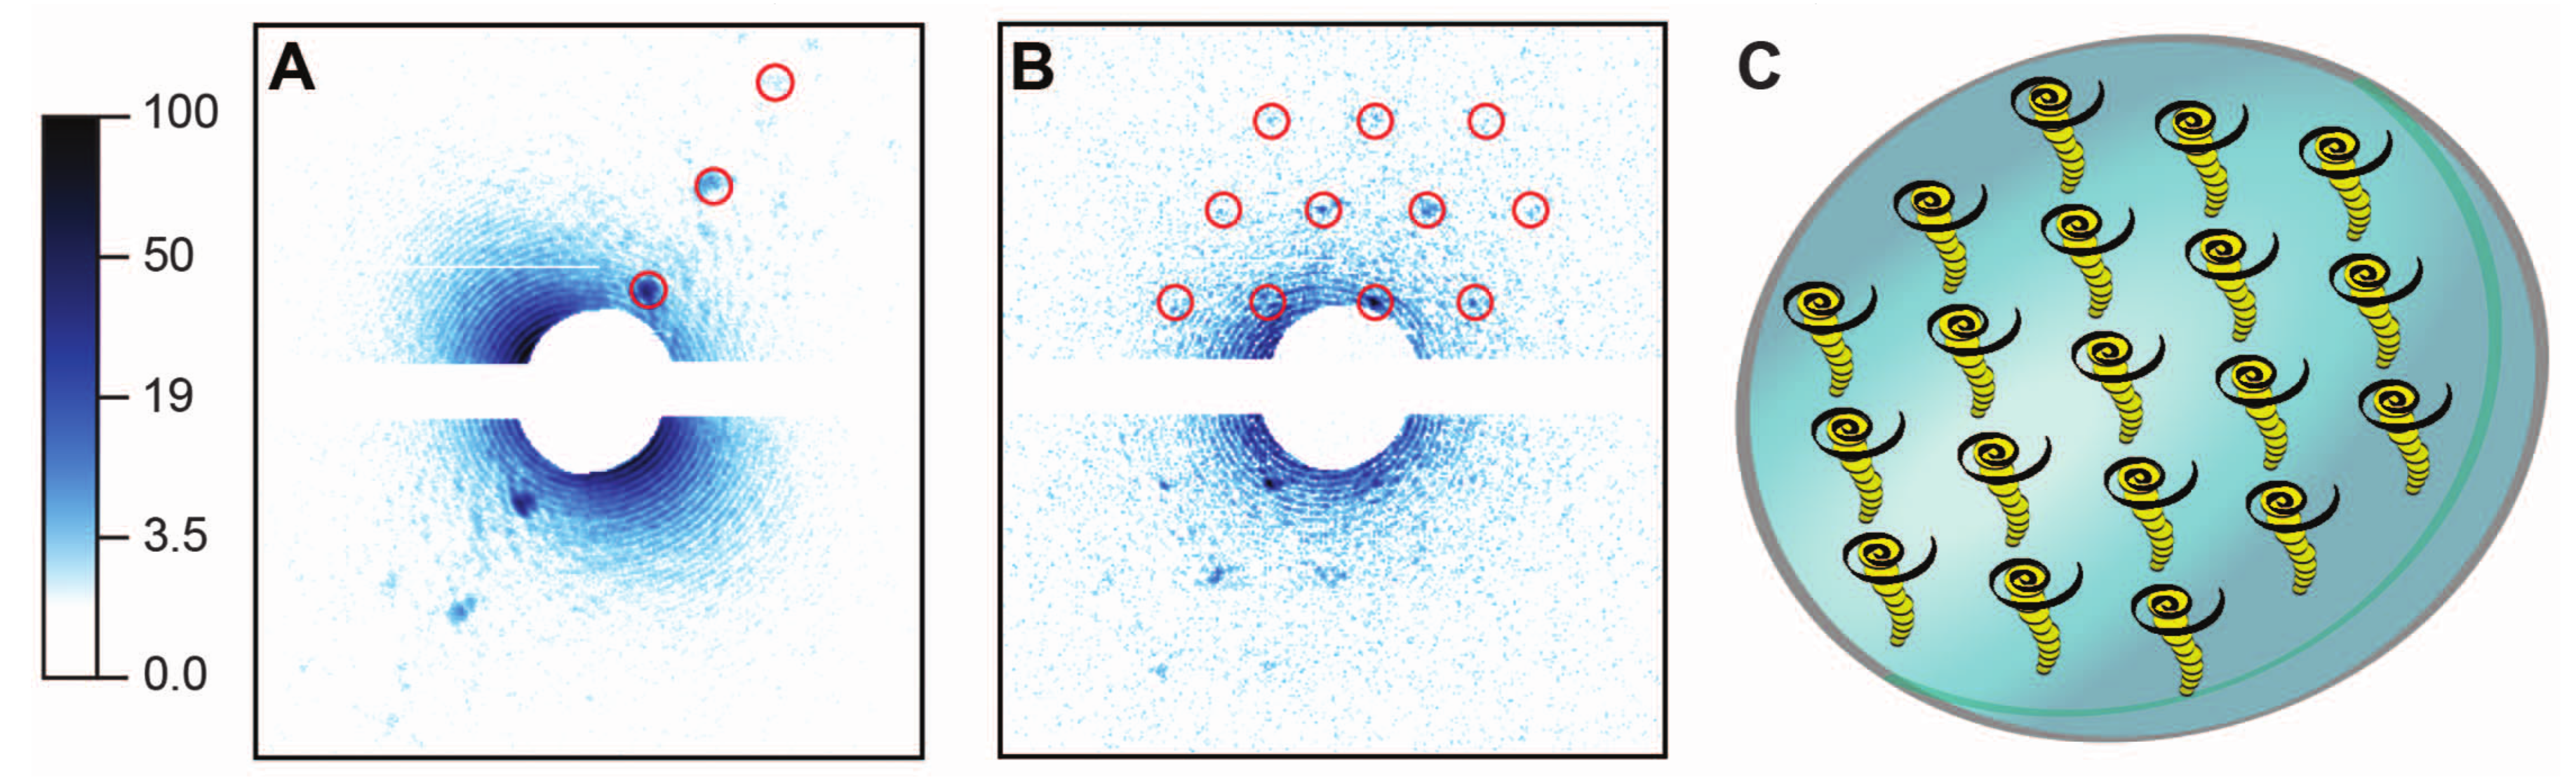
\includegraphics[width=\textwidth]{vortex-array}
			\caption{He droplets doped with Xe atoms. (A and B) X-ray diffraction images of doped droplets, displayed in a logarithmic intensity scale. (C) Droplet and embedded Xe clusters. Images in (A) and (B) correspond to tilted and parallel alignments of the vortex axes with respect to the incident x-ray beam, respectively.}
			\label{fig:vortex-array}
		\end{center}
	\end{figure}
\clearpage{\pagestyle{empty}\cleardoublepage}